
\let\negmedspace\undefined
\let\negthickspace\undefined
\documentclass[journal,12pt,twocolumn]{IEEEtran}
\usepackage{cite}
\usepackage{amsmath,amssymb,amsfonts,amsthm}
\usepackage{algorithmic}
\usepackage{graphicx}
\usepackage{textcomp}
\usepackage{xcolor}
\usepackage{txfonts}
\usepackage{listings}
\usepackage{enumitem}
\usepackage{mathtools}
\usepackage{gensymb}
\usepackage[breaklinks=true]{hyperref}
\usepackage{tkz-euclide} % loads  TikZ and tkz-base
\usepackage{listings}
\usepackage{gvv}
%
%\usepackage{setspace}
%\usepackage{gensymb}
%\doublespacing
%\singlespacing

%\usepackage{graphicx}
%\usepackage{amssymb}
%\usepackage{relsize}
%\usepackage[cmex10]{amsmath}
%\usepackage{amsthm}
%\interdisplaylinepenalty=2500
%\savesymbol{iint}
%\usepackage{txfonts}
%\restoresymbol{TXF}{iint}
%\usepackage{wasysym}
%\usepackage{amsthm}
%\usepackage{iithtlc}
%\usepackage{mathrsfs}
%\usepackage{txfonts}
%\usepackage{stfloats}
%\usepackage{bm}
%\usepackage{cite}
%\usepackage{cases}
%\usepackage{subfig}
%\usepackage{xtab}
%\usepackage{longtable}
%\usepackage{multirow}
%\usepackage{algorithm}
%\usepackage{algpseudocode}
%\usepackage{enumitem}
%\usepackage{mathtools}
%\usepackage{tikz}
%\usepackage{circuitikz}
%\usepackage{verbatim}
%\usepackage{tfrupee}
%\usepackage{stmaryrd}
%\usetkzobj{all}
%    \usepackage{color}                                            %%
%    \usepackage{array}                                            %%
%    \usepackage{longtable}                                        %%
%    \usepackage{calc}                                             %%
%    \usepackage{multirow}                                         %%
%    \usepackage{hhline}                                           %%
%    \usepackage{ifthen}                                           %%
  %optionally (for landscape tables embedded in another document): %%
%    \usepackage{lscape}     
%\usepackage{multicol}
%\usepackage{chngcntr}
%\usepackage{enumerate}

%\usepackage{wasysym}
%\documentclass[conference]{IEEEtran}
%\IEEEoverridecommandlockouts
% The preceding line is only needed to identify funding in the first footnote. If that is unneeded, please comment it out.

\newtheorem{theorem}{Theorem}[section]
\newtheorem{problem}{Problem}
\newtheorem{proposition}{Proposition}[section]
\newtheorem{lemma}{Lemma}[section]
\newtheorem{corollary}[theorem]{Corollary}
\newtheorem{example}{Example}[section]
\newtheorem{definition}[problem]{Definition}
%\newtheorem{thm}{Theorem}[section] 
%\newtheorem{defn}[thm]{Definition}
%\newtheorem{algorithm}{Algorithm}[section]
%\newtheorem{cor}{Corollary}
\newcommand{\BEQA}{\begin{eqnarray}}
\newcommand{\EEQA}{\end{eqnarray}}
\newcommand{\define}{\stackrel{\triangle}{=}}
\theoremstyle{remark}
\newtheorem{rem}{Remark}

%\bibliographystyle{ieeetr}
\begin{document}
%

\bibliographystyle{IEEEtran}


\vspace{3cm}

\title{
Question 1.5.7
}
\author{ EE22BTECH11051 - Sreekar Cheela 
}	

% make the title area
\maketitle

\newpage

%\tableofcontents

% Within an equation environment
1.5.7)
\\
\large The vertices of the given triangle are:
\begin{equation}
    \begin{array}{ccc}
        \begin{bmatrix}
            1 \\
            -1 \\
        \end{bmatrix};
        &
        \begin{bmatrix}
            -4 \\
            6 \\
        \end{bmatrix};
        &
        \begin{bmatrix}
            -3\\
            -5\\
        \end{bmatrix};
    \end{array}
\end{equation}
\\
Suppose the equations AB, BC and CA are respectively given by

 \large \begin{align}
    n_{i}^{T} x = c_i , i = 1,2,3
    \end{align}
\\
Then the equations of the angle bisectors are given as 
\\
\begin{align}
    \text {\large$\displaystyle \frac{\lvert n_{i}^{T} x - c_i  \rvert}{\lvert \lvert n_{i} \rvert \rvert}$}
\end{align}
 \\
\bigskip 
 From this equation, we get the angle bisector from B as:
  \begin{align}
        \begin{bmatrix}
            11 + 7\sqrt{\frac{61}{37}} \\
            1 + 5\sqrt{\frac{61}{37}}
        \end{bmatrix}^{T}
        \vec {x} = 2\sqrt{\frac{61}{37}}-38
    \end{align}
    
\\
From this equation, we get the angle bisector from C as:
  \begin{align}
        \begin{bmatrix}
            11 + 7\sqrt{61} \\
            1 - \sqrt{61}
        \end{bmatrix}^{T}
        \vec {x} = 2\sqrt{61}-38
    \end{align}

\bigskip
\begin{flushleft}
    The intersection of all the angle bisectors is given as the incentre.
Hence, the incentre can be found by finding the point of intersection of both
the angle bisectors.

On solving them, we get the incentre  as:
\end{flushleft}
\begin{align}
   I= \begin {bmatrix}
    \frac{-53-11\sqrt{37}+7\sqrt{61}+\sqrt{2257}}{12} \\ 
    \frac{5-\sqrt{37}+5\sqrt{61}-\sqrt{2257}}{12}
  \end{bmatrix}
\end{align}
\begin{flushleft}
    To find the radius of the incentre, we need to find the distance between 
    the incentre and any one of the sides. 
    \\
    Let us find the distance between BC line and I:
    \\
    BC line equation is given as:
    \bigskip
    \begin{align}
    \begin{bmatrix}
        7 \\
        5
    \end{bmatrix}^{T}
    \vec {x} = 2
    \end{align}
    \\
    Using the distance formula, we get the radius as:
    \\
    \begin{align}
    r = \frac{185+41\sqrt{37}-37\sqrt{61}-\sqrt{2257}}{6\sqrt{74}}
    \end{align}
    \\Hence the diagram is given as:
    \\
\end{flushleft}

\begin{figure}[h]
	\centering
	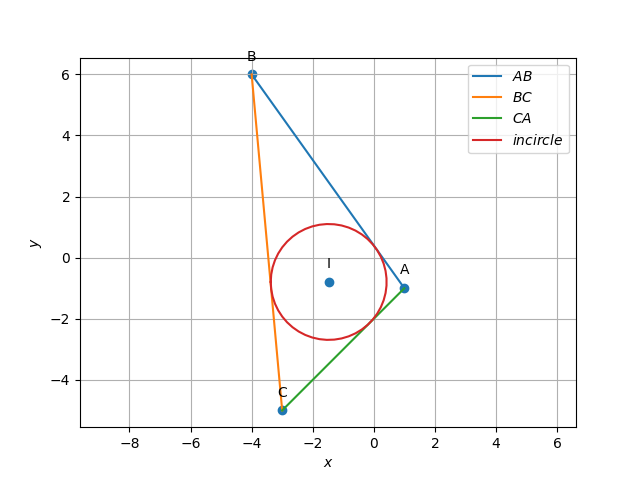
\includegraphics[width=\columnwidth]{./Diagram.png}
	\caption{Triangle with the incircle}
	\label{Incircle}
  \end{figure}

\renewcommand{\thefigure}{\theenumi}
\renewcommand{\thetable}{\theenumi}
%\renewcommand{\theequation}{\theenumi}

\end{document}
